%----------------------------------------
\begin{frame}[fragile]
  \frametitle{Instrumenting the generated code for monitoring} \small
\dejavubadge{}{instrumentation}{black!55}

\vspace{-0.2cm}
\fprime{} generates a C++ class per port type. In a verification build, each one gets a
subclass that records the call, then forwards it:

\vspace{0.1cm}
\begin{lstlisting}[style=cpp]
class OutputHeaterCommandPort : public OutputHeaterCommandPortBase {
  public:
    void invoke(const TempControl::HeaterState& heaterState) const {
      Fcheck::record(getObjName(), heaterState);
      OutputHeaterCommandPortBase::invoke(heaterState);
    }
};
\end{lstlisting}

\pause
\vspace{0.25cm}
The raw record: time, port, event id, timestamp, severity, argument bytes:

\vspace{0.1cm}
\begin{lstlisting}[style=shell]
92281991262,heaterActuator_eventOut_OutputPort[0],536903680,
1792172611.792976,x06,x0000000200000001
\end{lstlisting}

\pause
\vspace{0.25cm}
translated with the \fprime{} dictionary into a named event:

\vspace{0.1cm}
\begin{lstlisting}[language=qtl]
heaterActuator_STATE_CHANGED("FAULT", "ON")
\end{lstlisting}

\end{frame}

%----------------------------------------
\begin{frame}[fragile]
  \frametitle{A temporal property, in \dejavumt{}} \small
\dejavubadge{4}{violated}{red!75!black}

\vspace{0.3cm}
Using the event {\tt STATE\_CHANGED} from the generated vocabulary (slide 7):

\vspace{0.3cm}
\begin{lstlisting}[language=qtl]
// The actuator never goes straight from FAULT to ON: FAULT goes through OFF.
prop fault_cleared_before_heating :
  !heaterActuator_STATE_CHANGED("FAULT", "ON")
\end{lstlisting}

\end{frame}

%----------------------------------------
\begin{frame}[fragile]
  \frametitle{The violation, on a recorded run} \small
\dejavubadge{4}{violated}{red!75!black}

Scenario: heat until the heater has been on too long, then turn it on by hand.

\begin{lstlisting}[style=shell]
70.870 s  heaterActuator_STATE_CHANGED(ON, FAULT)
70.870 s  faultNotify
71.281 s  heaterController_MODE_CHANGED(MANUAL)
77.846 s  cmd_heaterController_HEATER_MANUAL_CMD(ON)
77.846 s  heaterCmd(ON)
77.846 s  heaterActuator_STATE_CHANGED(FAULT, ON)    <- violated here
\end{lstlisting}

\pause

\begin{block}{A real hazard}\small
The controller, in manual mode, allows the operator's ON straight on from FAULT.
The heater now runs with its {\bf safety limits off}.
\end{block}

\pause

\begin{block}{The same kind of bug as {\tt RESET\_STATISTICS}}\small
An operator command gets around the fault protection. The fix for the first bug,
found with \lean{}, did not cover this path.
\end{block}

\end{frame}

%----------------------------------------
\begin{frame}[fragile]
  \frametitle{Why FAULT $\to$ ON is dangerous: the latches} \small
\dejavubadge{4}{consequence}{black!55}

\vspace{-0.35cm}
\whereami{act}

Each limit has a {\bf latch}: a flag that, once set, stays set. A set latch means
``this fault has already been reported'', so the check does not fire every second.

\begin{lstlisting}[style=cpp]
if (dutyCycle > maxDutyCycle && !m_dutyCycleFaultTriggered) {
    setFaultState();                      // the heater goes to FAULT
    m_dutyCycleFaultTriggered = true;     // reported: stay silent from now on
}
...
if (oldState == FAULT && newState == OFF) {
    m_dutyCycleFaultTriggered = false;    // only FAULT -> OFF re-arms it
    m_continuousOnTimeFaultTriggered = false;
}
\end{lstlisting}

\pause

\begin{block}{The expected flow: FAULT $\to$ OFF $\to$ ON}\small
Going through OFF clears the latches, so both limits are checked again once the heater
is back on.
\end{block}

\end{frame}
%----------------------------------------
\begin{frame}
  \frametitle{Four properties, three levels} \small

\vspace{-0.25cm}
\begin{center}\small
\renewcommand{\arraystretch}{1.2}
\begin{tabular}{|c|>{\raggedright\arraybackslash}p{2.3cm}|>{\raggedright\arraybackslash}p{3.2cm}|>{\raggedright\arraybackslash}p{4.0cm}|}
\hline
\rowcolor{blue!10}
 & {\bf checked on} & {\bf property} & {\bf holds?}\\
\hline
1 & \lean{}\newline controller model & a hot reading turns the heater off
  & {\color{red!70!black}\bf false} as stated;\newline {\color{green!45!black}\bf true} given the proved\newline invariant \mbox{\tt hysteresis > 0}\\
\hline
2 & \lean{}\newline actuator model & a violated limit leads to FAULT, whatever else happens
  & {\color{red!70!black}\bf false}: operator sends\newline {\tt RESET\_STATISTICS}\\
\hline
3 & \lean{}\newline system model & a fault puts the controller in manual mode
  & {\color{green!45!black}\bf true}\\
\hline
4 & \dejavumt{}\newline the real code & the heater never goes directly from FAULT to ON
  & {\color{red!70!black}\bf false}: operator sends\newline {\tt HEATER\_MANUAL\_CMD(ON)}\\
\hline
\end{tabular}
\end{center}

\vspace{0.05cm}
{\small 2 and 4: an operator command gets around the fault protection.}

\end{frame}
%----------------------------------------
\begin{frame}
  \frametitle{What each method covers} \small

\vspace{0.1cm}
{\centering
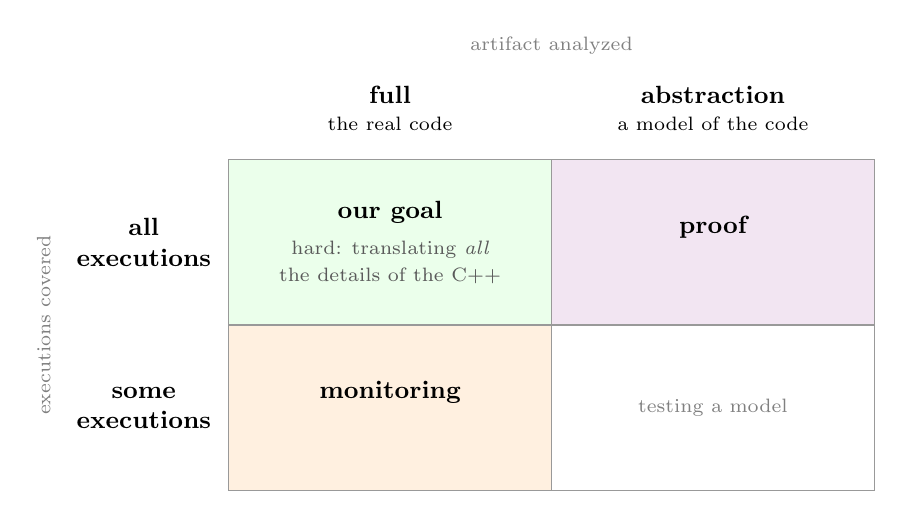
\begin{tikzpicture}[
  font=\small,
  cell/.style={draw=black!40, minimum width=4.1cm, minimum height=2.1cm, align=center},
  head/.style={font=\small\bfseries, align=center}
]
  % column heads: the artifact analyzed
  \node[head] at (2.05, 4.75) {full\\[-1pt]{\scriptsize\mdseries the real code}};
  \node[head] at (6.15, 4.75) {abstraction\\[-1pt]{\scriptsize\mdseries a model of the code}};
  \node[font=\scriptsize, gray] at (4.1, 5.55) {artifact analyzed};

  % row heads: the executions covered
  \node[head, anchor=east] at (-0.1, 3.05) {all\\executions};
  \node[head, anchor=east] at (-0.1, 0.95) {some\\executions};
  \node[font=\scriptsize, gray, rotate=90] at (-2.35, 2.0) {executions covered};

  \node[cell, fill=green!8] (fa) at (2.05, 3.05) {{\bf our goal}\\[2pt]{\scriptsize\color{black!65}hard: translating {\em all}}\\[-1pt]{\scriptsize\color{black!65}the details of the C++}};
  \node[cell, fill=violet!10] (pa) at (6.15, 3.05) {{\bf proof}\\[2pt]\lean{}};
  \node[cell, fill=orange!12] (fs) at (2.05, 0.95) {{\bf monitoring}\\[2pt]\dejavumt{}};
  \node[cell] (ps) at (6.15, 0.95) {{\color{gray}\scriptsize testing a model}};
\end{tikzpicture}\par}

\end{frame}
